\chapter{Background}

% WHAT IS A COMPILER 

To allow for a higher abstraction and higher level of resoning about 
algorithms new language has been developed. To be able to run these new languages
compilers has been built to "translate" the code down to machine code to run 
directly on hardware or to a lower level language to make use of their compiler. 

% GENERAL PIPELINE FIGURE

\begin{figure}[h!]
\label{fig:generalpipeline}
\centering
  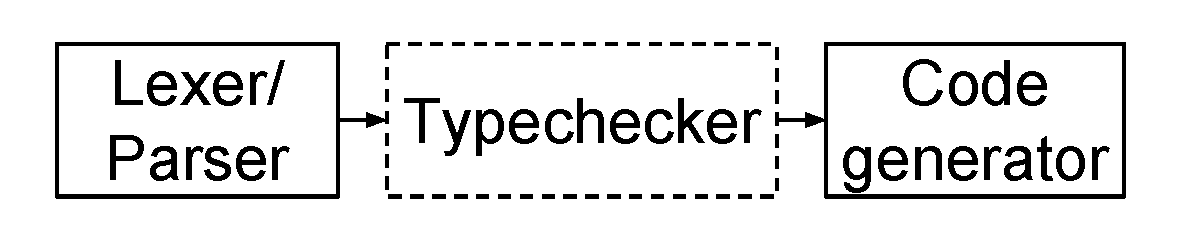
\includegraphics[width=0.6\pdfpagewidth]{figure/general-pipeline}
\end{figure}

% HOW IS A COMPILER BUILT 

When building a compiler it can be resembled to a pipe where text flows through 
while transformed into different representations and in the end outputted
to runnable code to either run on the computer itself or on a virtual machine
that emulates a computer. 

In figure ~\ref{fig:generalpipeline} you can see how the source flows through.
It should be noted that the typechecker is optional for a language. It can
fully rely on the grammar to expose errors, this will lead to a more expressive 
language while it may crash in execution due to type errors.

Now is Hopper really a transpiler or a translating compiler. Instead of 
outputting runnable code it outputs other code that is interpreted and compiled
by the Erlang compiler, erlc. With this the project could very much be 
simplified (ref to read more in discussion).

% OTHER SECTIONS

\section{Parsing source code} \label{sec:bnfc}

\todo{Assigned David}


A programming language is similar to a natural language in that it is described by a grammar. Programming languages are however different in that they are built from their grammar and are thus unambiguous.
The grammar describes ways in which the smaller pieces of the language can be put together to form bigger ones, often with more meaning. 

From this grammar a lexer is produced. The lexers job is to match all words in the source code to tokens in the grammar. For example in english the word 'boat' would match a noun token. This list of tokens is combined with a parser to make expressions or sentences. To make the language as expressive as possible one build up bigger expressions out of smaller expressions. This will create a tree structure that will be easier to work with. 

To save a lot of work, the lexer and parser can be automatically generated from a grammar written in \gls{bnf} using a tool called the \gls{bnfc} \cite{bnfc}, or BNFC for short. This tool is developed at Chalmers and used in earlier courses, meaning that multiple group members were already familiar with it.
\section{Renaming and simplifying}

\todo{Assigned DAvid}

While BNFC is a great tool to create a parse tree from raw text the resulting 
tree structure is very verbose with a lot of constructors. To simplify this a
renamer step is introduced in the pipeline. This step converts the parse tree
to our minimally designed \acrlong{ast} or \acrshort{ast} for short. 

% TODO I want these beside each other and a arrow in between
\begin{table}
\begin{lstlisting} 
f = if a                      f = case a of
      then b        =>              True  -> b
      else c                        False -> c
\end{lstlisting}
\caption{Simple transformation to a more general form}
\label{lst:renamer1}
\end{table}

In this step a few grammar rules could be translated to more general expressions
to simplify the AST and reduce the number of cases the typechecker need to cover, see
table \ref{lst:renamer1}.

The other part of the renamer module is to annotate the functions to where they
where exported from...

\section{Type checking}

Programmers inevitably make mistakes. While there are many tasks computers excel at, understanding the programmer's intent and detecting differences between it and the actual behavior of the programs they write is not one of them. To aid in the automatic detection of errors, semantic analysis may be used. One such kind of analysis is type checking, which is enabled by having a type system.

Type systems are formal systems which enable proof of absence of certain kinds of errors. They are typically defined in terms of inference rules.

Type systems can be used to help in rejecting invalid programs. They group values in the programming language into types, and specify rules about what is or what is not a valid interaction between them. For example, a type system might be defined to reject a program that tries to apply a number to a value as if it were a function.

There are two main kinds of type systems: dynamic and static. The most noticeable difference between dynamically and statically typed programming languages is whether type errors are discovered at run time or compile time.

Static type systems automatically detect type incorrect code at compile time, such as a program treating a Boolean as a list of Booleans. This allows the programmer to diagnose errors during the implementation phase. In contrast, dynamic type systems evaluate types during runtime, allowing the programmer to manipulate data in a more free manner.

An additional benefit of type systems is that they can be used as a means of specifying and documenting properties of a program in a concise way. Typically, a function may be annotated with a type signature which states the types of its arguments and its return type. 
\todo{Check this part again}

%For example, in Haskell a program which might have some side effects and returns a Boolean can be distinguished by its type (\texttt{IO Bool}) from a function which simply calculates a value of a pure mathematical proposition, which would be of type \texttt{Bool}.


% old liam stuff
% \section{Type checking} %Snälla konsultera mig innan stora ändringar av innehållet görs i Type checking-delar! %Åtminstone kommentera bara ut det som tas bort. %a) att det finns olika sorters semantisk analys påpekas i Compiler-delen %b) error/= exakt bug, dynamiska typsystem evaluerar inte typer att runtime etc. Programmers inevitably make mistakes. While there are many tasks computers excel at, understanding the programmer's intent and detecting differences between it and the actual behavior of the programs they write is not one of them. %To aid in the automatic detection of errors, semantic analysis may be used. One such kind of analysis is type checking, which is enabled by having a type system. To aid in the automatic detection of bugs, type systems have been devised. Type systems are formal rules governing what is and is not a valid program. They group values into types and specify what is and is not a valid interaction between those values. When a program type checks, the programmer can be assured that a common class of error is absent. For example, in most if not all languages it is not acceptable to use a number as if it were a function. The difference between dynamically typed languages such as Erlang and statically typed languages such as Haskell is whether the erroneous application is discovered at run time or compile time. An additional benefit of type systems is that they can be used as a means of specifying and documenting properties of a program in a concise way. For example, a program that sends and receives messages or has other side effects can be given a different type than one which simply calculates a value. In Section~\ref{sec:dai_tc}, we will demonstrate the advantages of using types to describe the kind of concurrent programs run on the BEAM virtual machine. %Type systems are formal systems which enable proof of absence of certain kinds of errors. They are typically defined in terms of inference rules. <<< Bra, ska se om jag kan arbeta in det här så att texten har flow. %Type systems can be used to help in rejecting invalid programs. %They group values in the programming language into types, and specify rules about what is or what is not a valid interaction between them. For example, a type system might be defined to reject a program that tries to apply a number to a value as if it were a function. %There are two main kinds of type systems: dynamic and static. The most noticeable difference between dynamically and statically typed programming languages is whether type errors are discovered at run time or compile time. \todo{Check this part again} %For example, in Haskell a program which might have some side effects and returns a Boolean can be distinguished by its type (\texttt{IO Bool}) from a function which simply calculates a value of a pure mathematical proposition, which would be of type \texttt{Bool}.

\section{Core Erlang and BEAM}

Core Erlang \cite{CoreErlangIntro} is an intermediate language in the Erlang compilation suite, mainly used for simplifying operations on Erlang source code. Such operations can include, but are not limited to: parsing, compiling and debugging. Some of the main purposes of Core Erlang are to be as regular as possible and to provide clear and simple semantics. The language is since release 8, released in 2001, an official part of the OTP/Open Source Erlang Distribution.

\Gls{beam} is the name of the Erlang virtual machine. Erlang and Core Erlang source code may be compiled to \texttt{.beam} files, which contain assembler instructions for the \gls{beam} virtual machine. These instructions are interpreted by the virtual machine at run time.

